\documentclass[border=10pt]{standalone}
\usepackage{pgfplots}
\usepgfplotslibrary{colormaps}
\pgfplotsset{trig format plots=rad}
\begin{document}
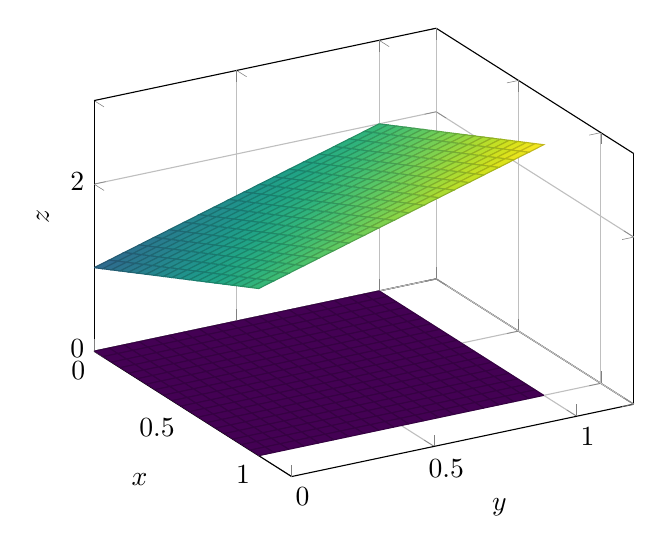
\begin{tikzpicture}
\begin{axis}[
    view={60}{30},
    xlabel=$x$, ylabel=$y$, zlabel=$z$,
    xmin=0, xmax=1.2, ymin=0, ymax=1.2, zmin=0, zmax=3,
    grid=major,
    colormap/viridis
]
% Surface z = 1 + x + y
\addplot3[surf, domain=0:1, y domain=0:1, samples=20] {1 + x + y};
% The region D in xy plane
\addplot3[patch, domain=0:1, y domain=0:1, samples=20] {0}; 
% Note: For simplicity, we will just plot the boundaries of the solid
\end{axis}
\end{tikzpicture}
\end{document}
